
\documentclass{cccg16}

\usepackage{amssymb, amsmath}
\usepackage{graphicx}
\usepackage{hyperref}
\usepackage[utf8]{inputenc}
\usepackage[T1]{fontenc}
\usepackage{lmodern}
\usepackage{hhline}
\usepackage{wrapfig}
\usepackage{subfig}
\usepackage{listings}
\usepackage{courier}
\usepackage{float}
\usepackage{color}

\usepackage{lipsum}

\DeclareMathOperator{\sign}{sign}
\DeclareMathOperator{\fma}{fma}
\DeclareMathOperator{\round}{round}
\def\Jack#1{{\bf [[#1]]}\ignorespaces}
%\def\Jack#1{\ignorespaces}%% uncomment to hide remarks
\def\Michael#1{{\bf \color{red} [[#1]]}\ignorespaces}
%\def\Jack#1{\ignorespaces}%% uncomment to hide remarks

\lstset{basicstyle=\ttfamily}

\title{On the Precision to Sort Line-Quadric Intersections}
\author{Michael Deakin \and Jack Snoeyink\thanks{School of Computer
    Science, University of North Carolina at Chapel Hill, {\tt
      mfdeakin@cs.unc.edu}, {\tt snoeyink@cs.unc.edu}}}

\index{Deakin, Michael}
\index{Snoeyink, Jack}

\begin{document}
\thispagestyle{empty}
\maketitle

\begin{abstract}
  We consider a subproblem of the task of exactly tracking a neutron
  moving along a given line segment through a CAD model with quadric
  surfaces, namely, how much more than the input precision is required
  to guarantee the correct ordering along the line segment of the
  intersections from a pair quadrics.  When the order of all but one
  pair of intersections is known, we show that a resultant can
  resolve the comparison using only half the precision that may be
  required to eliminate radicals by repeated squaring, and we compare
  the time and accuracy of our technique with converting to extended
  precision to calculate roots.
\end{abstract}

\section{Introduction}
In this paper, we are concerned with the points of line-quadric
intersections.  As a result, we need complimentary representations for
these objects.  Points are easiest to represent as a tuple~$(x, y,
z)$.  Lines are most easily representable with parametric equations of
the form~$l(t)=(m_x t + c_x, m_y t + c_y, m_z t + c_z)$.  This works
well with our representation of a point, because the result of this
equation is a point.  Quadric surfaces are not so easy to represent as
parametric equations, due to their non-linear nature.  Instead, it is
easier to represent them as an isosurface of the form~$Q(x, y,
z)=q_{xx} x^2 + q_{xy} xy + q_{xz} xz + q_x x + \dots + q_{zz} z^2 +
q_{z} z + q_c = 0$.  This fits well with our previous definitions, as
this equation takes points as inputs.  As a result, it is easy to
determine whether a point is on the surface and the line-quadric
intersection.

A line-quadric intersection is a point~$p=(x, y, z)$ computable from
the parametric line equation that satisfies the quadric surface
equation.  The parameter of the line specifying the point of
intersection can be computed by finding the roots of~$Q(l(t))=a t^2 -
2 b t + c$.  This is easiest to do with the quadratic equation, but
the result is not so useful for comparisons.  Directly using the
result of the quadratic equation for comparison has issues with
correctness when performed at the same precision as the coefficients
of the input line and quadric surfaces.

Correctness in this case is defined for a particular set of
inputs. \Jack{This first sentence adds nothing but the mistaken
  impression that Correctness has already been defined.  The next is
  easier if you've already mentioned representations above.  And we
  don't really want all things to be integers -- well scaled floating
  point is fine.  For now we can just say single, and assume that the
  exponents are close enough that making them equal does not lose
  bits.}  Specifically, a computation is said to be correct if for all
inputs which are integers when multiplied by $2^{-e}$ and are less
$2^p$, the rounded result of a series of additions, multiplications,
divisions, and square roots is exact.  The correctness of the computed
parameter can be ensured by increasing the precision of the
intermediate computations.  Because all inputs are integers, additions
can usually be computed exactly without any increase in precision.
Multiplication requires the precision to be increased to the sum of
the precisions of the input values.
% This is terrible!! Fix it!!!
Correctness requires the results of expressions to be exactly
representable in the final format, so in general the use of divisions
or square roots disqualifies a method from being correct.

% Not as terrible
When the sign of a computation is all that's required, a single square
root is permissible, as comparing the radicand and the square of the
other term will determine the sign of the result.
% Need a more precise way of saying this...
When multiple square roots are present, determining the sign is made
harder because the minimum number of bits required to reasonably
approximate the difference is unknown \cite{demaine33open}.  Luckily,
correctness of the sign computation can still be guaranteed if the
maximum possible rounding error is less than the magnitude of the
result.

In this work, we compare three different methods for computing the
order of line-quadric intersections.  These methods are specifically
developed for the case where only one pair of roots has a difference
which is potentially overwhelmed by the rounding errors in the
computation.  This is a notable limitation, but scenes of quadric
surfaces which can have more than one pair of ambiguous roots are rare
and should be dealt with specifically.

\section{Methods}
Three line-quadric intersection comparsion methods are evaluated in
terms of correctness, precision requirements, and FLOPs required.
These methods include the ``Approximate Comparison Method'', the
``Repeated Squaring Method'', and the ``Resultant Method''.

\subsection{Approximate Comparison Method}
The approximate comparison method computes, for $i\in\{1, 2\}$, the
roots~$r_i^\pm=({b_i\pm\sqrt{b_i^2-a_ic_i}})/{a_i}$ approximately by
computing each operation.  The order of the approximate roots can be
calculated exactly as~$\sign(r_1^\pm-r_2^\pm)$.

Though this method will usually give correct orders, it clearly does
not guarantee them, since intermediate computations, such as the
square roots, cannot be computed exactly for all inputs.

Because this method cannot guarantee correctness, any precision
increases are optional and only serve to increase the likelihood of
computing the correct order of intersections.

Because no effort was spent to guarantee correctness, this method
requires very little computation.  Computing the both roots requires
only $12$ FLOPs, and computing the sign of the difference requires
only one more.  The roots can also be reused in cases where 

\subsection{Repeated Squaring Method}
This method computes~$\sign(r_1^\pm-r_2^\pm)$ with some algebraic
manipulations to eliminate division and potentially bad square root
operations.  We eliminate these operations by using the following
property:~$\sign(y)=\sign(x)\sign(x\cdot y)$.  Divisions can be
removed by applying this directly, in this case bringing us
to~$\sign(a_1 a_2)\sign(a_1 a_2 (r_1^\pm-r_2^\pm))$.  One of the
square roots can be replaced by multiplying by $r_1^\pm-r_2^\mp$,
bringing us to~$\sign(a_1 a_2)\sign(a_1 a_2
(r_1^\pm-r_2^\mp))\sign(a_1^2 a_2^2 (r_1^\pm - r_2^\pm) (r_1^\pm -
r_2^\mp))$.  When simplified, the final sign is computed
from~$a_2^2b_1^2-2a_1a_2^2c_1+2a_1^2a_2c_2-a_1a_2b_1b_2\pm
\sqrt{(a_1a_2b_2-a_2^2b_1)^2(b_1^2-4a_1c_1)}$. This is sufficient to
compute the correct result, as the simplified equation contains only
one square root, multiplications, and additions.

Despite the work done, it's not immediately clear that this leads to a
correctly computable method.  The remaining issues are present in the
other sign computation with square roots. $\sign(r_1^\pm-r_2^\mp)$ is
not correctly computable in general.  However, because we are
computing $\sign(r_1^\pm-r_2^\pm)$, we know that $r_1^\pm, r_2^\pm$
are the only pair roots for which the sign of the difference cannot be
computed exactly.  This resolves all issues with guaranteeing
correctness for this computation.

Though this method is correct, it requires a large increase in
precision to correctly compute the sign. The terms outside of the
square root can be computed correctly by increasing the precision
to~$4\times$ the coefficients precision.  The precision increases
to~$8\times$ after squaring for comparison to the radicand.  The terms
inside the radicand also require~$8\times$ the coefficients precision
to be computed correctly.

This method also requires a large number of FLOPs.  Computing the
unambiguous sign of the difference of the roots requires 15 FLOPs
total.  Correctly computing the final sign requires another 24 FLOPs.
Unfortunately, because many of the computed terms require coefficients
from both polynomials, they cannot be reused if a quadric needs to be
compared multiple times.  The main thing that can be reused is the
discriminant, which only reduces the number of FLOPs by 8.
Fortunately, cases where a quadric is close enough to multiple
quadrics for this to become a significant issue are rare.

\subsection{Resultant Method}
Another method for computing the order of two intersections involves
computing the resultant for their respective polynomials.  The
resultant of two polynomials can be computed by taking the determinant
of the Sylvester Matrix.  The Sylvester Matrix for
polynomials~$P(t)=p_m t^m + \dots + p_0$ and~$Q(t)=q_n t^n + \dots +
q_0$ is defined in Equation \ref{eq:sylv}.
\begin{equation}
  S_{PQ}=\begin{pmatrix}
    p_m & \dots & & p_0 & 0 & & 0\\
    0 & p_m & \dots & & p_0 & & 0\\
    & \ddots & & & & \ddots\\
    0 & 0 & & p_m & \dots & & p_0\\
    q_n & \dots & & q_0 & 0 & & 0\\
    0 & q_n & \dots & & q_0 & & 0\\
    & \ddots & & & & \ddots\\
    0 & & q_n & \dots & & q_0\\
  \end{pmatrix}
  \label{eq:sylv}
\end{equation}
where~$P$ and~$Q$ are polynomials of one parameter and with orders~$m$
and~$n$, respectively \cite[Section~3.5]{cheeyap}.

The determinant of the Sylvester matrix is defined to be the resultant
of the two polynomials.  Given the roots~$a_i, b_i$ of~$P$ and~$Q$,
respectively, the resultant can also be computed as shown in Equation
\ref{eq:resultant}. \cite[Section~6.4]{cheeyap}.
\begin{equation}
  res(P, Q)=p_m^n q_n^m \prod_{i=1}^m\prod_{j=1}^n (a_i-b_j)
  \label{eq:resultant}
\end{equation}

The two methods of computing the resultant provides us with an extra
method of computing the sign of one of the differences of the two
roots.  Since we are concerned only with the signs of the differences,
the actual value doesn't matter.  Thus, if one of the differences is
too close to zero for comfort, we can compute the correct sign for it
from the signs of the other differences and the sign of the
determinant.  Equation \ref{eq:resultant} lets us write Equation
\ref{eq:signresult}.

\begin{equation}
  \sign(res(P, Q)) =
  \sign(p_m^n)\sign(q_n^m)\prod_{i=2}^m\prod_{j=1}^n[\sign(a_i-b_j)]
  \label{eq:signresult}
\end{equation}

Without loss of generality, let us be concerned with the sign
of~$a_1-b_1$.  The sign of~$a_1-b_1$ can then be computed as shown in
Equation \ref{eq:signroot}

\begin{figure*}
  \begin{align}
    \sign(a_1-b_1)=\sign(res(P, Q))\sign(p_m^n)\sign(q_n^m)
    \prod_{i=2}^m\prod_{j=2}^n[\sign(a_i-b_j)\sign(a_1-b_j)\sign(a_i-b_1)]
    \label{eq:signroot}
  \end{align}
\end{figure*}

For simplicity of computation, instead of performing many
multiplications, we need to count only the number of negatives on the
right hand side of this equation.  If there are an even number of
negatives, then the undetermined sign will be positive.  If there are
an odd number of negatives, the undetermined sign will be negative.
Since we are concerned with the intersections of lines with quadric
surfaces, we know our polynomials will be of order~$2$, and thus that
the signs of~$p_2^2$ and~$q_2^2$ will be positive and can be ignored.

It should be immediately apparent that computing the determinant can
be done more cheaply than correctly computing the sign of the
differences of roots of the polynomials.  Computing the roots of the
polynomials requires seven additions and multiplications, plus the
expensive square root and two divisions.  For reference, it has been
shown that a square root costs approximately the same number of
operations as~$\frac{3}{2}$ additions at the same precision
\cite{karatsuba}.  To compute the roots, two multiplications and an
addition are computed at 6 times the precision of the input.  The
square root and two additions are computed at 12 times the initial
precision.  The two divisions are computed at 24 times the initial
precision.  To actually perform the comparison, one final subtraction
is required at 24 times the initial precision. This means each
comparison requires only 1 FLOP, with an initialization cost of 10
FLOPs per intersection.

On the other hand, computing a determinant of a 4x4 matrix costs about
120 multiplications.  This is clearly too expensive, so we specialize
for the Sylvester matrix.  Computing the determinant of the Sylvester
matrix itself would naively take~$35$ FLOPs for each comparison.  We
can do better by computing the per-polynomial values shown in Equation
\ref{eq:sylvpoly}.  Since these values are solely determined by one of
the polynomial's coefficients, we compute these once at first use, and
store them for whenever we need to make future comparisons.  This
brings us to 11 FLOPs per comparison, with an initialization cost of 7
FLOPs per intersection.

\begin{figure*}
  \begin{equation*}
    \Delta=\begin{vmatrix}
    a_1 & b_1 & c_1 & 0\\
    0 & a_1 & b_1 & c_1\\
    a_2 & b_2 & c_2 & 0\\
    0 & a_2 & b_2 & c_2\\
    \end{vmatrix}=
    a_1^2 c_2^2 + c_1^2 a_2^2 + b_1^2 a_2 c_2 + b_2^2 a_1 c_1 -
    b_1 c_1 a_2 b_2 - a_1 b_1 b_2 c_2 - 2 a_1 c_1 a_2 c_2
  \end{equation*}
  \begin{align}
    \alpha_i=a_i^2,\,\, \gamma_i=c_i^2,\,\,
    \delta_i=a_i b_i,\,\, \epsilon_i=a_i c_i,\,\, \zeta_i=b_i c_i,\,\,
    D_i=b_i^2-\epsilon_i,\,\,
    i\in {1, 2}\\
    \Delta = \alpha_1 \gamma_2 + \gamma_1 \alpha_2 +
    D_1 \epsilon_2 + \epsilon_1 D_2 - \zeta_1 \delta_2 -
    \delta_1 \zeta_2
  \label{eq:sylvpoly}
  \end{align}
\end{figure*}

This reduction theoretically makes this method slightly cheaper than
computing the roots of the polynomial at higher precision.  Computing
the determinant this way always requires six multiplications and five
additions at 4 times the precision of the coefficients.  Computing the
per-polynomial values requires six multiplications and one subtraction
at 6 times the precision of the input.

Since we are concerned only with the signs of the differences of
roots, no evaluation of the product of the known differences of the
roots is needed.  Thus, no other increase of precision is required for
the computation of the sign of the difference of the final pair of
roots.

\section{Evaluation}
\subsection{Evaluation Methods}
The approximate comparison and resultant methods were implemented in a
C++ program for evaluation.  MPFR was used to implement the increased
precision in both cases.

To ensure the results from both methods were consistent, the ordered
lists of roots were divided into regions based on a relative threshold
heuristic.  This heuristic put an upper limit on the largest bit that
could change in a single region.  To compensate for gradual changes in
a region, this heuristic depended only on the largest root seen in the
region to this point.  If the number of roots in the region was
different for the two methods, the results are listed as possibly
being erroneous.  Note that this method does not verify that the
regions contain the same quadrics; as the quadrics in each region can
vary based on the order of previously seen quadrics.

Once the line was generated, the intersections and their order were
computed along with some statistics.  These statistics were the amount
of time the sorting process took, the number of comparisons made at
higher precision, and whether the results of the two algorithms
approximately matched.  The C++ STL sort function was used to sort the
computed list of intersections, and the POSIX clock\_gettime function
was used for timing.

Since we implemented the methods in such a way that they implicitly
expect a quadratic polynomial, we have a limitation on the types of
quadric surfaces allowed in the test scenes.  Any scene which is used
to evaluate the speed of the methods in our test must ensure a line
will either intersect a surface twice, intersect it once with a
multiplicity of two, or not intersect it at all.  This is guaranteed
for most surfaces, but can occur on rare occasion with parabolic
cylinders, hyperbolic paraboloids, and elliptic paraboloids.  To
prevent this issue from occurring, we do not include these types of
quadric surfaces in our test scenes.  We also do not include any
linear planes in our scenes.

\subsection{Test Scenes}
To compare the methods, several scenes of quadric surfaces were
created.  These scenes, shown in figure \ref{fig:testScenes}, were
composed of surfaces which were mostly constrained within the unit
cube centered at~$(0.5, 0.5, 0.5)$.  To actually perform the tests,
10000 random lines were generated.  These lines were generated with
intercepts positioned within the unit cube to make close intersections
more likely.

\begin{figure}
  %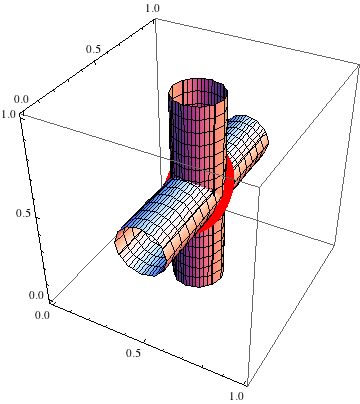
\includegraphics[width=0.5\textwidth]{imgs/cylinder_model_planeless.png}
  %\vspace{1mm}
  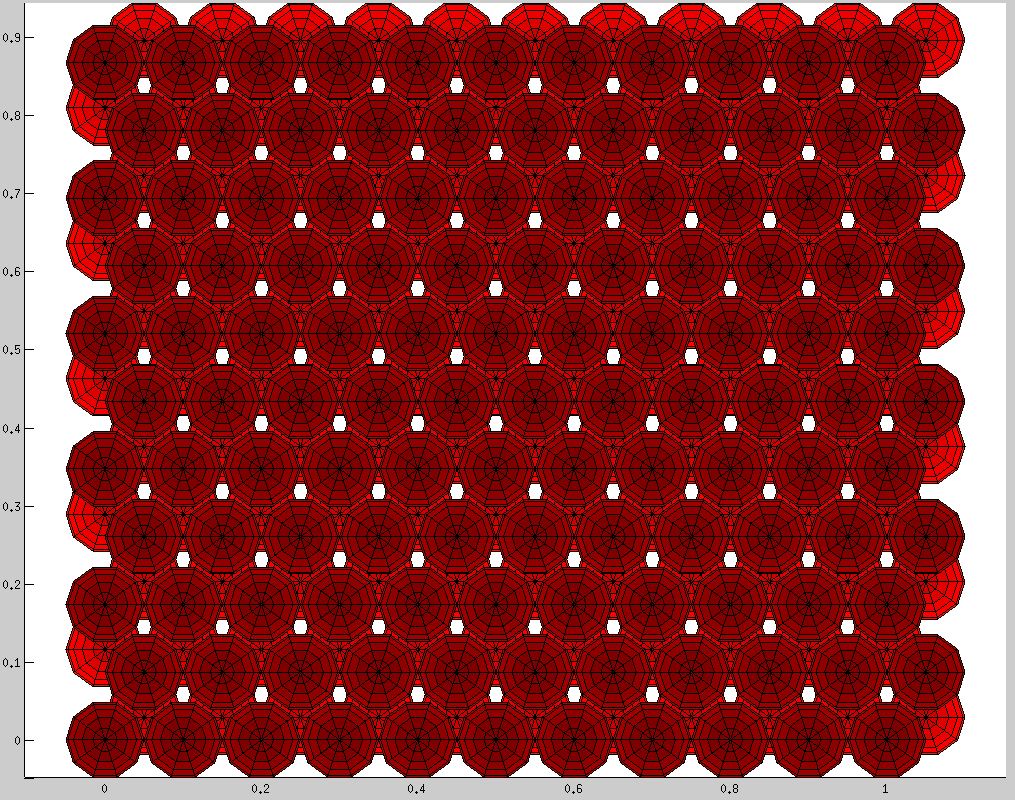
\includegraphics[width=0.5\textwidth]{imgs/packedSpheres.png}
  
  \vspace{5mm}
  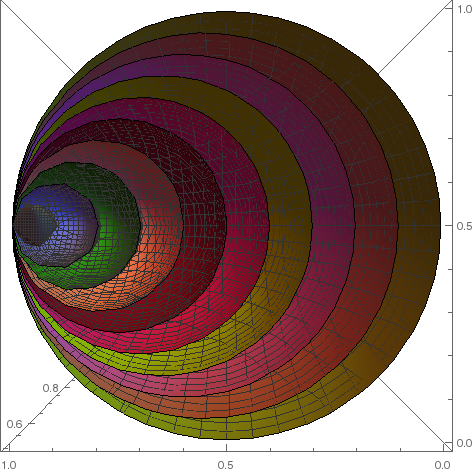
\includegraphics[width=0.5\textwidth]{imgs/hardEllipsoidsSingle.png}
  \caption{Test Scenes, from Top to Bottom:
    %{\bf Test Cylinders};
    {\bf Packed Spheres};
    {\bf Shifted Ellipsoids}}
  \label{fig:testScenes}
\end{figure}

\subsection{Analysis}
To analyze the results, we computed the least squares linear fit of
the timing data.  For the Packed Ellipsoids, we used the number of
comparisons made as our independent variable, and computed a linear
coefficient for it along with a constant term.  For the set of Shifted
Ellipsoids, we were able to aggregate the test results for each type
of scene.  This allowed us to fit the line to two independent
variables; the number of comparisons made, and the number of quadric
surfaces in the scene.  Fitting the time it takes to make a comparison
to a linear relationship makes sense, as the bulk of the sorting time
is taken up by performing these comparisons.  It also makes sense for
the time to be linearly related to the number of quadrics in the
scene, as the cached values are only computed once for each quadric,
and are likely to significantly affect the time a comparison takes.

\subsection{Hardware}
Three computers were used to test the implementations.  The first
computer has a Core i3 M370 processor with 2 cores and a 3 MB cache.
This processor does provide not a hardware implementation of FMA.
This computer has 4 GB of DDR3 memory clocked at 1 GHz.  It is running
an up to date installation of Arch Linux with version 4.4 of the
kernel.  GCC 5.3 was used to compile the code for these tests.  For
these tests, the performance manager was set to keep the CPU clock at
2.4 GHz, and the process was run with a nice value of -20.

The second computer has two Xeon E5-2643 processors with 4 cores and
10 MB caches.  This processor does not provide a hardware
implementation of FMA.  This computer has 32 GB of DDR3 memory running
with a 1.6 GHz clock.  It is running Ubuntu 14.04 with version 3.13 of
the kernel, and uses GCC 5.2 to compile the code for these tests.
These tests were run with the default performance manager with a
maximum CPU clock of 3.3 GHz, along with a nice value of -20.

The third computer has a Core 2 Duo E6550 processor with two cores and
a 4 MB cache.  This processor does not provide a hardware
implementation of FMA.  This computer has 8 GB of DDR2 memory clocked
at 667 MHz.  It is running an up to date installation of Gentoo Linux
with version 4.0 of the kernel.  GCC 5.3 was used to compile the code
for these tests.  For these tests, the performance manager was set to
keep the CPU clock at 2.3 GHz, with a nice value of -20.

To get a better estimate of the relative performance of the two
computers, the Geekbench benchmark was employed to estimate the
processor speeds.  The Ubuntu computer had a single core floating
point score of 2730.  The Arch computer had a single core floating
point score of 1702.  The Gentoo computer had a single core floating
point score of 1408.  On average, the Ubuntu computer was capable of
about 1.6 times more FLOPS than the Arch computer, and 1.9 times more
FLOPS than the Gentoo computer.

\section{Experimental Results}
The results of the experiments are shown in Table \ref{tab:times}.
Each method took approximately the same amount of time to process each
quadric, though the resultant method consistently took the longest.
This is because the resultant method caches some of the intermediate
values when the first comparison is made, shifting some portion of the
cost from the ms/Comp term to the ms/Quadric term.  The
amount that is shifted is determined by how many quadrics a random
line can be expected to intersect, and how many ambiguous orderings a
single line-quadric intersection will be involved in.  The increased
precision approximation method also took longer than the machine
precision approximation method for essentially the same reason as the
resultant method.  It's not entirely clear why it took less time than
the resultant method, as it performs harder computations on the first
use of the quadrics roots than the resultant.

The second term is approximately how much time each comparison takes.
Not surprisingly, the machine precision method took very little time
per comparison.  This is because nearly all of it's work is done on a
per quadric basis - the roots are calculated for each quadric once,
and only a subtraction is required for each comparison. The resultant
method also performed significantly better than the increased
precision method on a per comparison basis.  This is as expected,
given the reduction in the amount of precision, the number of FLOPs
required, and the lack of operations such as square roots and
divisions.

The constant term appears to be rather meaningless when we measure the
ms/Quadric term.  This is good, because it shows that when the
ms/Quadric term is not measured, that is mainly what the constant term
consists of.  Thus, we expect, and observe the same results as in the
ms/Quadric term.  It also means there are probably not any other terms
which should be considered.

\begin{figure}
  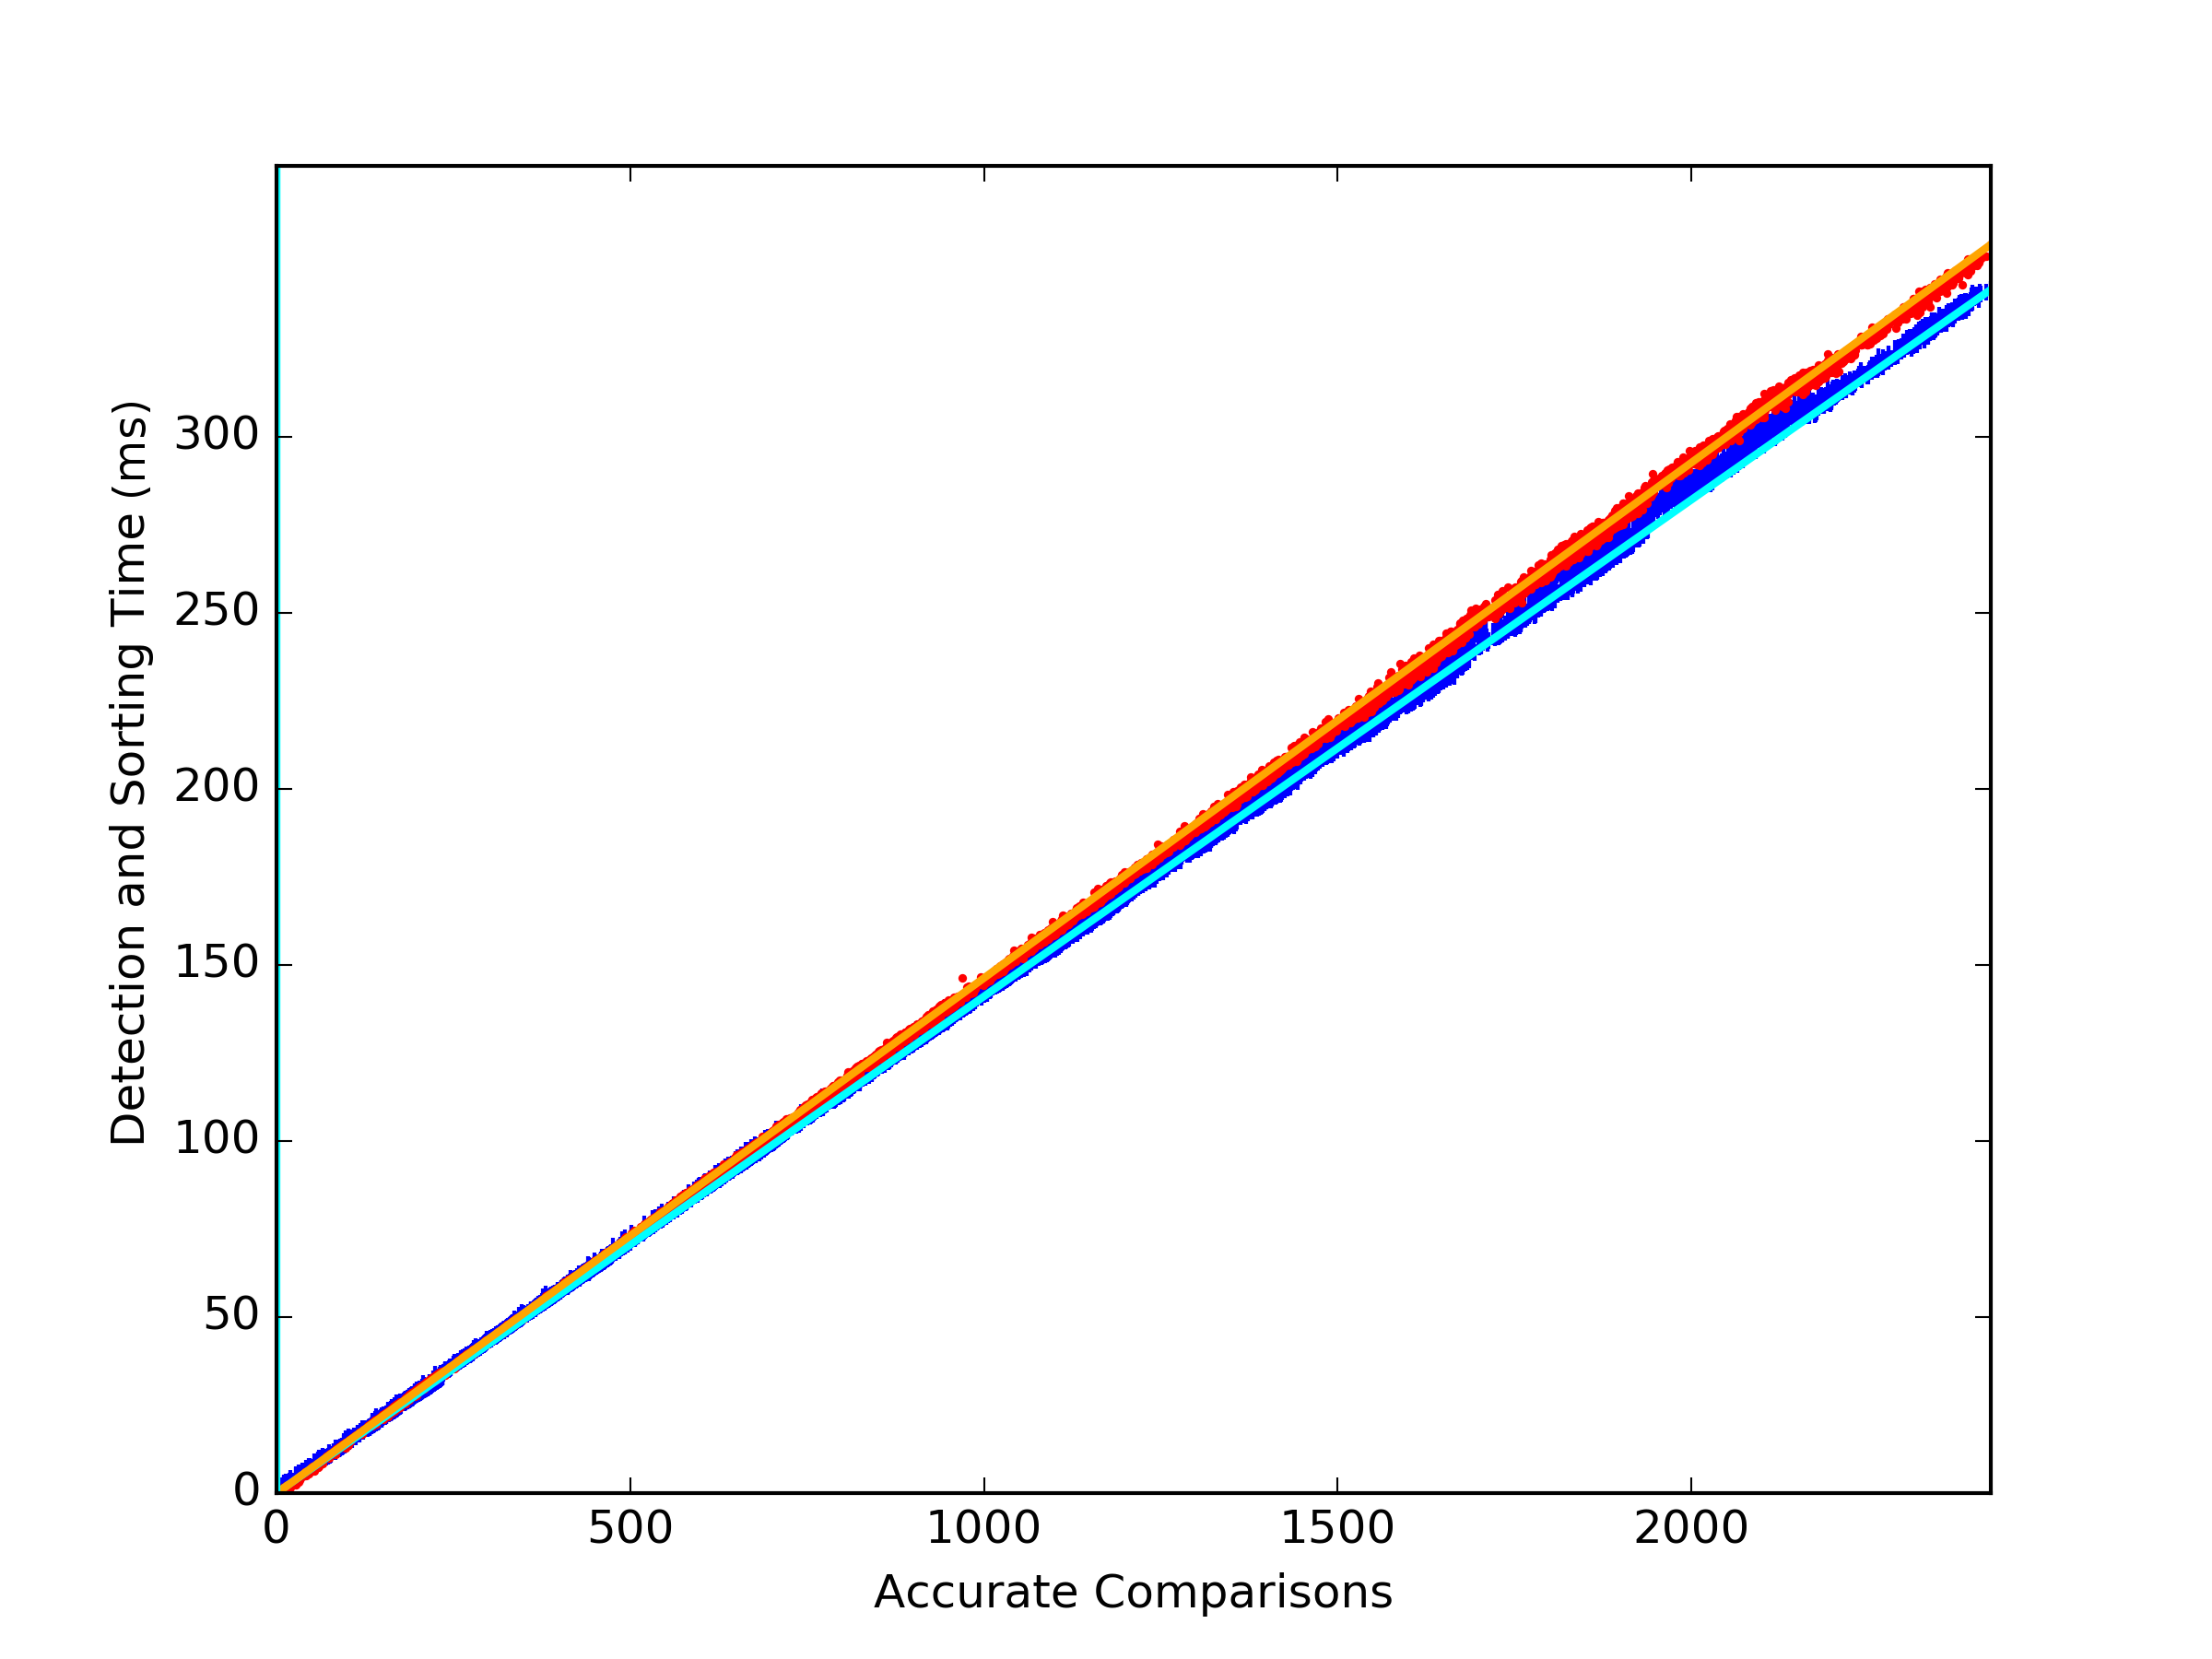
\includegraphics[width=0.55\textwidth]{imgs/hardEllipsoidsSingle_gentoo_adjusted.png}
  \caption{Typical plot of Number of Comparisons vs. the Evaluation
    Time (ms); {\bf Red: Approximation Method at $24\times$ the
      Input Precision}; {\bf Green: Approximation Method at Input Precision}; {\bf Blue: Resultant Method}}
  \label{fig:linefit}
\end{figure}

Figure \ref{fig:linefit} shows a plot of the results from one of the
tests.  It appears to confirm our expectation that the time required
is linearly coorelated with the number of precision increases.

\begin{table}[p]
  \captionsetup{oneside, margin={1cm,0cm}, width=\textwidth}
  \caption{Timing Results of the Approximate Comparison and Resultant Comparison}
  \label{tab:times}
  \begin{tabular}{|l|l|ll|lll|l|}
\hline
Machine & Scene & Method & Disagreements & $\frac{\text{ms}}{\text{Quadric}}$ & $\frac{\text{ms}}{\text{Comparison}}$ & Constant $\text{ms}$ & Residual ($\text{ms}^2$)\\
\hhline{|=|=|==|===|=|}
Ubuntu & Packed & Increased Prec. & \hphantom{1}--- & -- & \hphantom{-}0.06823 & \hphantom{-}5.399 & \hphantom{10}1194.8288\\
& Spheres & Approximate & 103 & -- & -0.009685 & \hphantom{-}5.399 & \hphantom{10}1161.2192\\
&& Resultant & \hphantom{1}89 & -- & \hphantom{-}0.05687 & \hphantom{-}5.408 & \hphantom{10}1194.1208\\
\hline
& Nested & Increased Prec. & \hphantom{1}--- & 0.004163 & \hphantom{-}0.07064 & -0.002835 & \hphantom{1}28554.479\\
& Spheres & Approximate & \hphantom{1}13 & 0.004098 & \hphantom{-}0.000255 & -0.001070 & \hphantom{10}2806.9520\\
&& Resultant & \hphantom{10}0 & 0.004309 & \hphantom{-}0.05846 & \hphantom{-}0.007079 & \hphantom{1}32989.590\\
\hline
Arch & Packed & Increased Prec. & \hphantom{1}--- & -- & \hphantom{-}0.1364 & \hphantom{-}4.893 & \hphantom{100}334.98312\\
& Spheres & Approximate & \hphantom{1}85 & -- & \hphantom{-}0.000304 & \hphantom{-}4.942 & \hphantom{100}316.04740\\
&& Resultant & \hphantom{1}75 & -- & \hphantom{-}0.1139 & \hphantom{-}4.921 & \hphantom{100}327.24112\\
\hline
& Nested & Increased Prec. & \hphantom{1}--- & 0.003835 & \hphantom{-}0.1157 & \hphantom{-}0.05856 & 582387.69\\
& Spheres & Approximate & \hphantom{1}11 & 0.003864 & \hphantom{-}0.000591 & -0.01970 & \hphantom{10}7533.7867\\
&& Resultant & \hphantom{10}1 & 0.004088 & \hphantom{-}0.09580 & \hphantom{-}0.05074 & 558251.79\\
\hline
Gentoo & Packed & Increased Prec. & \hphantom{1}--- & -- & \hphantom{-}0.1711 & \hphantom{-}4.522 & \hphantom{100}255.93646\\
& Spheres & Approximate & \hphantom{1}94 & -- & \hphantom{-}0.004651 & \hphantom{-}4.513 & \hphantom{100}256.48723\\
&& Resultant & \hphantom{1}84 & -- & \hphantom{-}0.1424 & \hphantom{-}4.551 & \hphantom{100}258.49985\\
\hline
& Nested & Increased Prec. & \hphantom{1}--- & 0.003670 & \hphantom{-}0.1639 & \hphantom{-}0.02020 & \hphantom{1}62122.965\\
& Spheres & Approximate & \hphantom{1}19 & 0.003562 & \hphantom{-}0.000446 & -0.003482 & \hphantom{10}3327.8361\\
&& Resultant & \hphantom{10}0 & 0.003892 & \hphantom{-}0.1372 & \hphantom{-}0.06507 & 176409.02\\
\hline
\end{tabular}

\end{table}

\section{Conclusion}
In this paper we showed how the resultant method can improve the
accuracy in comparing a single line-quadric intersections at a much
lower cost than simply increasing the amount of precision.  This
method also satisfies our notion of correctness, unlike the
approximation method.  This method is applicable in many cases and can
provide significant improvements to performance over the regular
method of increasing precision.

\Michael{I've got the method for when multiple orders are ambiguous,
  but haven't mentioned it.  It's an obvious place to go, just not
  very frequently useful.  Should I include this as future work?}

A remaining problem to solve is computing the intersection order
correctly when the order of mutliple roots is undetermined.  When a
shared root is detected, it would be easy to determine if the other
roots are shared as well with the discriminants.  Because the terms of
the discriminants are fast to compute exactly, they could be compared
exactly relatively easily.  Since the discriminant is quadratically
related to the distance between the roots of a polynomial, this will
tell us exactly if both roots are shared, and if not, the order of the
non-shared roots.

\section{Acknowledgements}
We would like to acknowledge support from a contract with the Bettis
Atomic Power Laboratory.

\bibliographystyle{plain} \bibliography{resultantmethod}
\end{document}
